\clearpage{}
\subsection{Logical View}
\label{sec:logical-view-parent}
The purpose of the Logical View is to give interested stakeholders an overview of the different modules of the system, 
and how they communicate between each other. 
   

\begin{figure}
	\centering
		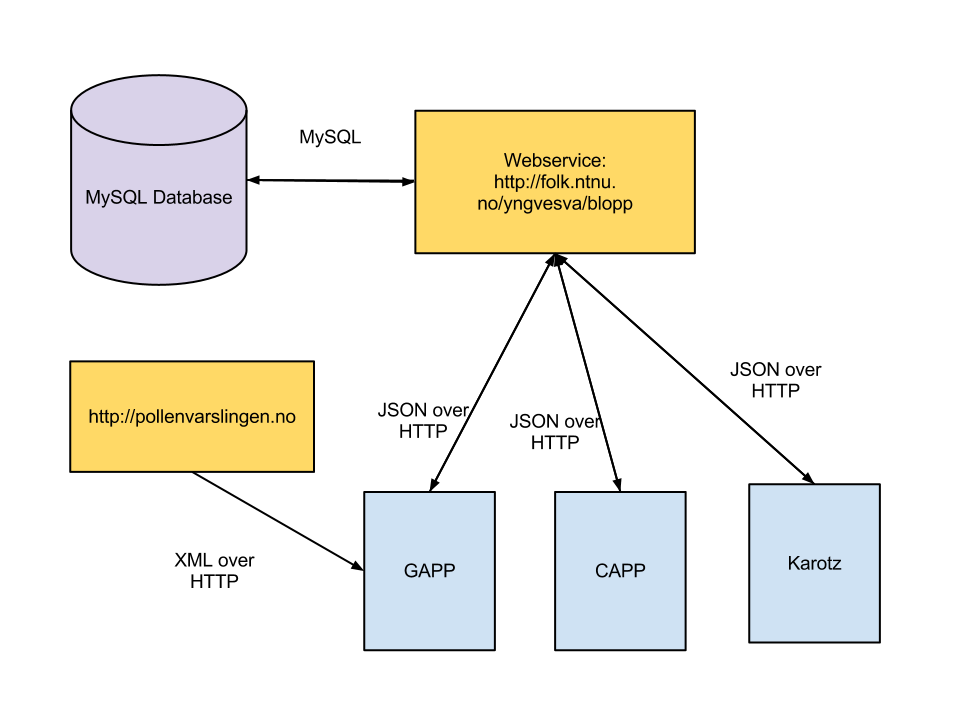
\includegraphics[width = 11.5 cm]{Pictures/ArchPictures/logicview.png}
	\caption{Logical View for the system} 
	\label{fig:package-diagram-system}
\end{figure}

Figure \ref{fig:package-diagram-system} shows the package diagram for the system. 

The locial view shows the different modules of the system, and the communication protocols between them. 


As mentioned in Section \ref{sec:pollencast}, NAAF provides a pollen forecast at \url{http://pollenvarslingen.no} which we intended to integrate with our system. It is currently not connected,
because the pollen forecast only operates during pollen season. It is however an important component for GAPP, and should be put in use during further development. 
We have worked around this fact in order to give the prototype a bit more content. This is described in more details in Appendix \ref{chap:class-diagram}.
 

The webservice is an important part that ties the different applications together. It required a lot of hours spent on developing it during the early stages, but
it definetly paid off later. 
There were several reasons to provide a webservice for the application:
\begin{itemize}
  \item Karotz only provides HTTP GET and POST methods for communicating over network,
  \item Our database server allocated at mysql.stud.ntnu.no is only available from NTNU's LAN (Local area network), which in practice means that a phone that is not connected to eduroam would get access to the database. 
  \item All MySQL queries are allocated at the same place.
\end{itemize}


% This package diagram is the top level folder structure for GAPP. Since we are using a MySQL-database hosted at NTNU, we had to work around
% some problems considering that we don't have access to the database unless we are connected to NTNU's LAN. The solution to this problem 
% introduced the webservice, which serves the purpose as a middle man between GAPP and the database. From this webservice, we retrieve data from over HTTP,
% using JSON. We also post data to the database through the package called jsonposters. Note that there is no security in this webservice, 
% which needs to be changed before deployment.
%  
% The diagram also shows a package called xmlfeed. This package serves the purpose of parsing XML into Java-code. Originally, the idea was to
% use pollenvarslingen.no's XML-feed. However, this feed is not running at the autumn and winter, so we replicated that XML-feed in our own 
% ``dummy''-feed \footnote{This XML-file is hosted at: \url{http://folk.ntnu.no/yngvesva/blopp/dummy/PollenForecast.xml}}.
% 
% This xml-document has similar structure as the original feed, only with test data for the sake of the prototype and proof-of-concept. 
% We have developed GAPP using MVC as our main architectural pattern. However, implementing MVC in Android is a bit different from other applications. 
% In Android, the activities serves both as a View and as the Controller (because of the touch screen).
% Thus, the Activity package will include all Activities needed, like \code{MainMenu} and \code{DistractionActivity}, etc. In addition, in order to render listviews, gridviews, etc.
% we need to make custom adapters, hence introducting the adapters-package. 
% 
% The package views only contains the relevant classes for the Log. We need this package since \code{CalendarView} is rendered programatically (taking
% dates into consideration when rendering). 
% 
% The repositories-package is not used at the moment, but we figured it would be a good idea to introduce it here for the future development team. Before the system is deployed,
% we expect that the database server will be changed. The repositories-package is a brief start on which functionality that needs to be implemented if the application
% is going to communicate directly with the database. It is by no means ready to put in use, but it is a start.   
% 
% We'll explain the content in each package more detailed in the Development View.
% 
% \subsubsection{Logical View -- CAPP}
% \begin{figure}
% 	\centering
% 		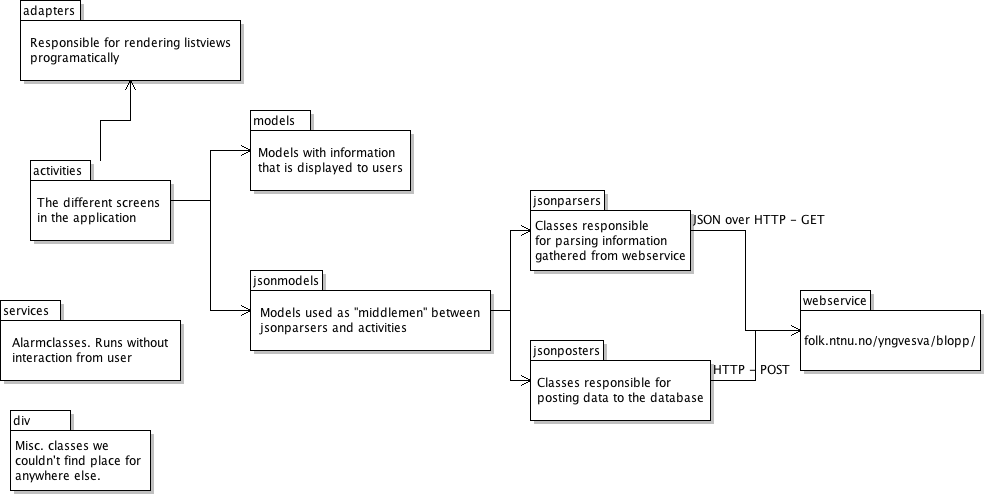
\includegraphics[width = 11.5 cm]{Pictures/ArchPictures/capparchpictures/capp_package_diagram}
% 	\caption[GAPP package diagram]{Package diagram for CAPP. A line from package X to package Y describes an association from X to Y. }
% 	
% 	\label{fig:package-diagram-system-capp}
% \end{figure}
% 
% Figure \ref {fig:package-diagram-system-capp} shows the logical view (package diagram) for CAPP. CAPP has about the same architecture as GAPP. 
% The main difference is the ``services'' package. A service in Android is a task that is done without any interactions from the user. In our case, 
% we use the services-package to update alarms once the phone is turned on, and on request. CAPP uses the same database and webservice as GAPP, and 
% a lot of the parsers in this application are equal to those found in GAPP.
% 
% \subsubsection{Logical View -- Karotz}
%  \begin{figure}
%  	\centering
%  		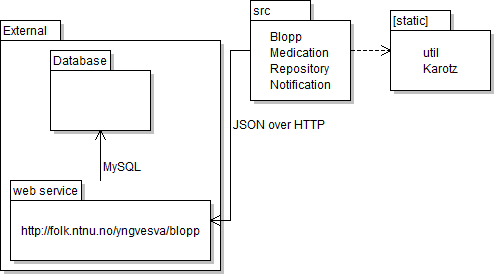
\includegraphics[width=12cm]{Pictures/ArchPictures/KarotzPackageDiagram}
% 	\caption[Karotz package diagram]{Package diagram for the Karotz application}
% 	\label{fig:package-diagram-system-karotz}
%  \end{figure}
% 
% Figure \ref{fig:package-diagram-system-karotz} shows the logical view of the Kartoz application. The only internal package in the Karotz application 
% is named ``src''. It contains all the main logic for the application, including a repository for connecting to the webservice for connecting to the 
% database, a notification module for setting alarms, a medication module for doing distraction; and a ``Blopp'' module for keeping track of everything. 
% There is an additional package in the diagram named ``\lbrack{}static\rbrack{}''. It contains the Karots class which is inherited from the OS and 
% contains various utilities for controlling output and recieveing input for the robot. It has been extended with some helper methods in the 
% implementation. There is also a ``util'' class which contains additional utility methods that do not belong in ``Karotz''. At last, there is indicated 
% an ``External'' package, which symbolizes all the external services the application connects to. In the case of the Karotz application, this includes 
% only the web service that connects to the database.